\documentclass[a4paper, 12pt]{article}%тип документа

%%%Библиотеки
	%\usepackage[warn]{mathtext}	
	\usepackage[T2A]{fontenc} % кодировка
	\usepackage[utf8]{inputenc} % кодировка исходного текста
	\usepackage[english,russian]{babel} % локализация и переносы
	\usepackage{caption}
	\usepackage{listings}
	\usepackage{multirow}
	\usepackage{amsmath,amsfonts,amssymb,amsthm,mathtools}
	\usepackage{wasysym}
	\usepackage{graphicx}%Вставка картинок правильная
	\usepackage{float}%"Плавающие" картинки
	\usepackage{wrapfig}%Обтекание фигур (таблиц, картинок и прочего)
	\usepackage{fancyhdr} %загрузим пакет
	\usepackage{lscape}
	\usepackage{xcolor}
	\usepackage[normalem]{ulem}
	\usepackage{hyperref}

%%%Конец библиотек




%%%Настройка ссылок
	\hypersetup
	{
		colorlinks=true,
		linkcolor=blue,
		filecolor=magenta,
		urlcolor=blue
	}
%%%Конец настройки ссылок


%%%Настройка колонтитулы
	\pagestyle{fancy}
	\fancyhead{}
	\fancyhead[L]{Лабораторная работа}
	\fancyhead[R]{Талашкевич Даниил, группа Б01-008}
	\fancyfoot[C]{\thepage}
%%%конец настройки колонтитулы

\newcommand{\const}{\mathrm{const}}
\newcommand{\rref}[1]{(\ref{#1})}
\newcommand{\isotope}[2]{$ ^{#2}\mathrm{#1} $}
\newenvironment{comment}{}{}
\newcommand{\picref}[1]{рис. \ref{#1}}
\newcommand{\mbf}{\mathbf}
\newcommand{\gmm}{$\gamma $}
\newcommand{\btt}{$\beta $}
\newcommand{\dlt}{$\delta $}
\newcommand{\Equip}[3]{
	
	\item{\bf #1:} $\Delta = \pm #2\; #3$}
\newcommand{\equip}[1]{
	
	\item{\bf #1}}
\newcommand{\labname}{Исследование энергетического спектра \btt-частиц и определение их максимальной энергии при помощи	магнитного спектрометра} 	% название пиши здесь
\newcommand{\labnum}{5.4.2}		% номер вводи здесь
\renewcommand{\epsilon}{\varepsilon}
\renewcommand{\phi}{\varphi}
\newcommand{\angstrom}{\text{\AA}}

							\begin{document}
						%%%%Начало документа%%%%


%%%Начало титульника
\begin{titlepage}

	\newpage
	\begin{center}
		\normalsize Московский физико-технический институт \\(госудраственный 			университет)
	\end{center}

	\vspace{6em}

	\begin{center}
		\Large Лабораторная работа по квантовой физике\\
	\end{center}

	\vspace{1em}

	\begin{center}
		\large \textbf{Измерение коэффициента ослабления потока $\gamma$-лучей в веществе и определение их энергии [5.1]}
	\end{center}

	\vspace{2em}

	\begin{center}
		\large Талашкевич Даниил Александрович\\
		Группа Б01-008
	\end{center}

	\vspace{\fill}

	\begin{center}
	Долгопрудный \\2022
	\end{center}
	
\end{titlepage}
%%%Конец Титульника



%%%Настройка оглавления и нумерации страниц
	\thispagestyle{empty}
	\newpage
	\tableofcontents
	\newpage
	\setcounter{page}{1}
%%%Настройка оглавления и нумерации страниц


					%%%%%%Начало работы с текстом%%%%%%

\section{Аннотация}

	\textbf{Цель работы:} c помощью сцинтилляционного счетки измерить линейные коэффициенты ослабления потока $\gamma$-лучей в свинце, железе и алюминии; по их велечине определить энергию $\gamma$-квантов.

\subsection{Теоретическая часть}
	Гамма-лучи возникают при переходе возбужденных ядер из одного энергетического состояния в другое, более низкое. Энергия $\gamma$-квантов обычно заключена между несколькими десятками килоэлектронвольт и несколькими миллионами электрон-вольт. Гамма-кванты не несут электрического заряда, их масса равна нулю. Проходя, через вещество, пучок $\gamma$-квантов постепенно ослабляется. Ослабление просходит по експоненциальному закону, который может быть записан в следующей форме:
	\begin{equation}
		\label{eq1}
		I = I_0 e^{-\mu l},
	\end{equation}
	где $I$, $I_0$ -- интенсивности прошедшего и падающего излучений; $l$ -- длина пути, пройденного пучком $\gamma$-лучей; $\mu$ -- коэффициент ослабления потока в веществе.
	
	Ослабление потока $\gamma$-лучей, происходящее при прохождении среды, связано с тремя эффектами: фотоэлектрическим поглощением, комптоновским рассеянием и с генерацией электрон-позитронных пар.
	
	В случае опытов, поставленных в хорошей геометрии, при прохождении $\gamma$-лучей через вещество меняет только количество, но не энергия $\gamma$-квантов в пучке, так что коэффициент $\mu$, характеризующий поглощение $\gamma$-квантов в веществе, не зависит от длины пути. Обозначим через $-dN$ число $\gamma$-квантов, выбывших их пучка на пути $dl$. Это число пропорционально имеющемуся их числу $N$ и пройденному пути $dl$. Cледовательно,
	\begin{equation}
		\label{eq2}
		-dN = \mu N \, dl.
	\end{equation} 
	Интегрируя уравнение~(\ref{eq2}) от нулевой толщины до заданной, получим
	\begin{equation}
		\label{eq3}
		N = N_0 e^{-\mu l}.
	\end{equation}

	Вообще говоря, в плохой геометрии, когда рассеянные под небольшими углами $\gamma$-кванты остаются в пучке, их спектр с прохождением вещества меняется, поэтому формула~(\ref{eq1}) непреминима. Однако в этом случае она работает лучше, чем можно было ожидать.
	
	В данной работе коэффициент ослабления $\mu$ измеряется в хорошей геометрии. Из формулы~(\ref{eq3}) имеем:
	\begin{equation}
		\tag{$\star$}
		\label{formula}
		\mu = \frac{1}{l} \ln \frac{N_0}{N}.
	\end{equation}

	Для определения коэффициента ослабления нужно, таким образом, измерить толщтну образца $l$, число падающих частиц $N_0$ и число частиц $N$, прошедших через образец.
	
\subsection{Экспериментальная установка}
	Схема установки, исползуемой в работе, показана на рис.~\ref{fig:ustanovka1}. Свинцовый коллиматор выделяет узкий почти параллельный пучок $\gamma$-квантов, проходящий через набор поглотителей П и регистрируемый сцинтиляцонным счетчиком. Сигналы от счетчика усиливаются и регистрируются пересчетным прибором ПП. Высоковольтный выпрямитель ВВ обеспечивает питание сцинтилляционного счетчика.
	
	\begin{figure}[h!]
			{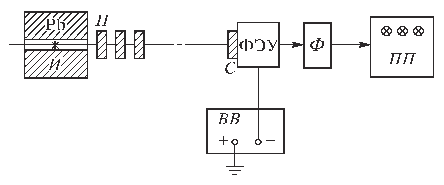
\includegraphics[scale=1.5]{ustanovka1.pdf}}    
		\caption{Блок-схема установки, используемой для измерения коэффициентов ослабления потока $\gamma$-лучей.}\label{fig:ustanovka1}
	\end{figure}

	При недостаточно хорошей геометрии в результаты опытов могут вкрасться существенные погрешности. В реальных установках всегда имеется конечная вероятность того, что $\gamma$-квант провзаимодействует в поглотителе несколько раз до того, как попадет в детектор (пути таких квантов показаны на рис.~\ref{fig:ustanovka2}). Чтобы уменьшить число таких случаев, в данной работе сцинтилляционный счетчик расположен на большом расстоянии от источиника $\gamma$-квантов, а поглотители имеют небольшие размеры. Их следует устанавливать за коллиматорной щелью на некотором расстоянии друг от друга, чтобы испытавшие комптоновское рассеяние и выбывшие из прямого потока кванты с меньшей вероятностью могли в него вернуться.

	\begin{figure}[h!]
			{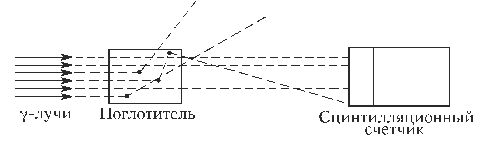
\includegraphics[scale=1.5]{ustanovka2.pdf}}    
		\caption{Схема рассеяния $\gamma$-квантов в поглотителе.}\label{fig:ustanovka2}
	\end{figure}
	
\section{Ход работы}	
	
	\subsection{Экспериментальные данные}
		В условиях нашего эксперимента необходимо учитывать фон, поэтому
		\begin{equation*}
			N_0 = n_0 - n_\text{фон}, \ N = n - n_\text{фон}.
		\end{equation*}
		
		
		\begin{table}[!h]
		\begin{center}
			\caption{Измерение фона и потока $\gamma$-излучения в воздухе.}
			\label{table:exp1}
			\begin{tabular}{|c|c|c|}
				\hline
				& $t$, с & $n$    \\ \hline
				$n_{\text{фон}}$ & 10    & 170   \\ \hline
				$n_0$            & 10     & 139843 \\ \hline
			\end{tabular}
		\end{center}
		\end{table}
		
		
	

		\begin{table}[!h]
		\begin{center}
			\caption{Результаты измерений.}
			\label{table:exp2}
			\begin{tabular}{|c|c|c|c|c|c|c|c|c|c|c|c|}
				\hline
				\multicolumn{3}{|c|}{Алюминий} & \multicolumn{3}{c|}{Железо} & \multicolumn{3}{c|}{Свинец} & \multicolumn{3}{c|}{Пробка} \\ \hline
				$l$, см   & $t$, с   & $<n>$     & $l$, см  & $t$, с  & $<n>$    & $l$, см  & $t$, с  & $<n>$    & $l$, см     & $t$, с    & $<n>$       \\ \hline
2,01      & 10      & 90184  & 1,01     & 10     & 77631 & 0,49     & 10     & 74789 & 1,97        & 10        & 139843    \\ \hline
4,02      & 10      & 58592  & 2,04     & 10     & 41492 & 0,97     & 10     & 41581 & 3,92        & 10        & 136826    \\ \hline
5,99      & 10      &  38074& 3,02     & 10     & 23703 & 1,45     & 10     & 23430 & 5,91        & 10        & 133850    \\ \hline
7,99      & 10      & 24498 & 4,03     & 10     & 13304 & 1,90     & 10     & 13986 & 7,92        & 10        & 131576    \\ \hline
10,02     & 10      & 16575  & 5,03     & 10     & 7609  & 2,35     & 10     & 8351  & 9,78        & 10        & 129176    \\ \hline
			\end{tabular}
		\end{center}
		\end{table}
		
	
		Здесь $<n>$ -- это усредненное значение кол-ва частит, тк мы измеряли это значение несколько раз. Отметим, что при повторном измерении результаты измерений количества частиц $n$ отличались в среднем на 3\% от значений в табл.~\ref{table:exp2}. Поэтому относительная погрешность $n$ будет порядка 3\%. Длина $l$ была измерена достаточно точно штангенциркулем и $\sigma_l / l < 1\%$, где $\sigma_l = 0,01$ см.
		 
		 
	\newpage
	\subsection{Обработка результатов}
		Для определения коэффициента ослабления $\mu$ в различных веществах небходимо построить графики  зависимостей $\ln N_0/N$ от $l$. Погрешность вычисления натурального логарифма можно оценить следующим образом:
		\begin{equation*}
			\sigma_{\ln} = \frac{1}{N_0/N} \sigma_{N_0/N} = \sqrt{\left(\frac{\sigma_{N_0}}{N_0}\right)^2+\left(\frac{\sigma_{N}}{N}\right)^2} \approx \sqrt{\left(\frac{\sigma_{n_0}}{n_0}\right)^2+\left(\frac{\sigma_{n}}{n}\right)^2} = 0,05\sqrt{2} \approx 0,07.
		\end{equation*}
		
		\begin{table}[!h]
		\begin{center}
			\caption{Результаты вычислений.}
			\label{table:exp3}
			\begin{tabular}{|c|c|c|c|c|c|c|c|}
				\hline
				\multicolumn{2}{|c|}{Алюминий} & \multicolumn{2}{c|}{Железо} & \multicolumn{2}{c|}{Свинец} & \multicolumn{2}{c|}{Пробка} \\ \hline
				$l$, см    & $\ln N_0/N$, с    & $l$, см   & $\ln N_0/N$, с  & $l$, см   & $\ln N_0/N$, с  & $l$, см       & $\ln N_0/N$, с      \\ \hline
2,01       & 0,45              & 1,01      & 0,59            & 0,49      & 0,59            & 1,97          & 0,01                \\ \hline
4,02       & 0,85              & 2,04      & 1,16            & 0,97      & 1,09            & 3,92          & 0,03                \\ \hline
5,99       & 1,26              & 3,02      & 1,74            & 1,45      & 1,67            & 5,91          & 0,06                \\ \hline
7,99       & 1,67              & 4,03      & 2,31            & 1,90      & 2,22            & 7,92          & 0,08                \\ \hline
10,02      & 2,07              & 5,03      & 2,85            & 2,35      & 2,79            & 9,78          & 0,11                \\ \hline
			\end{tabular}
		\end{center}
		\end{table}
		
	
		По данным таблицы~\ref{table:exp3} были построены прямые (рис. \ref{fig:graph}), наклоны которых согласно формуле~(\ref{formula}) есть линейные коэффициенты ослабления $\mu$ потока $\gamma$-излучения в веществе.
	
\newpage
	
		\begin{figure}[h!]
			\centering{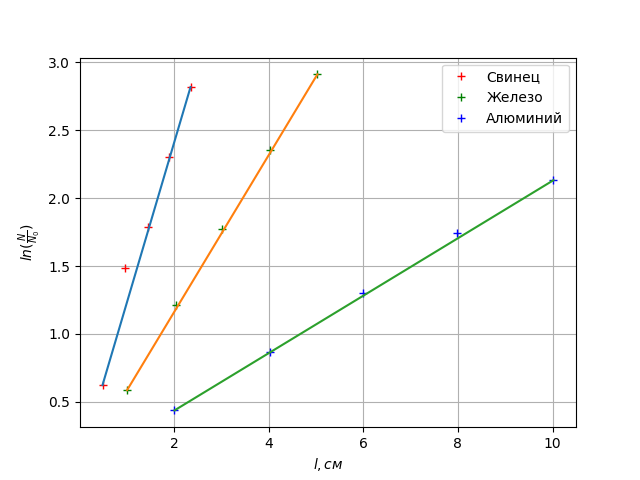
\includegraphics[scale=0.9]{all.png}}
			\caption{Графики зависимостей $\ln N_0/N$ от $l$ для различных материалов.}\label{fig:graph}
		\end{figure}
			
		Имеем:
		\begin{table}[!h]
		\begin{center}
			\caption{Наклоны прямых.}
			\label{table:final}
			\begin{tabular}{|c|c|c|c|}
				\hline
				& Pb          & Fe         & Al                         \\ \hline
				$\mu$, $10^{-3}\cdot \text{см}^{-1}$ & $1132\pm11$ & $561\pm 4$ & $201,7\pm 0,7$ \\ \hline
			\end{tabular}
		\end{center}
		\end{table}

	
\newpage
\section{Вывод}
	В настоящей лабораторной работе с помощью сцинтилляционного счетчика были измерены (табл.~\ref{table:final}) линейные коэффициенты ослабления $\mu$ потока $\gamma$-лучей в свинце, железе, алюминии и в некотором веществе <<X>>, которое внешне напоминало дсп. Среднюю энергию излучения, испускаемого источником, можно определить по следующей справочной таблице, приведенной в приложении лабораторного практикума по общей физике <<Квантовая физика>>:
	\begin{table}[!h]
	\begin{center}
		\caption{Коэффициенты поглощения $\gamma$-лучей в различных веществах (в~см$^{-1}$).}
		\label{table:spravocka}
		\begin{tabular}{|c|c|c|c|}
			\hline
			$E_\gamma$, МэВ & Pb    & Fe    & Al    \\ \hline
			0,6             & 1,349 & 0,605 & 0,210 \\ \hline
			0,8             & 0,982 & 0,526 & 0,184 \\ \hline
		\end{tabular}
	\end{center}
	\end{table}

	Видно, что полученные нами значения коэффициента ослабления потока $\mu$ для каждого вещества лежат в диапазоне энергий от 0,6 МэВ до 0,8 МэВ, поэтому средняя энергия излучения есть $E_\gamma = 0,7$ МэВ.
	
	Заметим, что наклоны прямых на рис.~\ref{fig:graph} по мере роста заряда ядра увеличиваются. Это связано с природой ослабления $\gamma$-лучей при их прохождении в веществе: фотоэлектрическое поглощение, комптоновское рассеяние, генерация электрон-позитронных пар. Так как $E_\gamma = 0,7 \ \text{МэВ} < 2mc^2$ = 1,02 МэВ, то в нашем случае фотон не может превратиться в электрон-позитронную пару. Комптоновское рассеяние происходит на свободных или слабосвязанных электронах, поэтому, очевидно, сечение не зависит от заряда ядра, откуда $\mu_k \propto Z$. Фотоэффект же в отличии от Комптоновского рассеяния происходит на атоме, и, естественно, что в этом случае сечение уже будет зависеть от заряда ядра. Вообще говоря, строгий квантово-механический рассчет приводит к результату $\sigma_\text{ф} \propto Z^5$. Таким образом, коэффициент ослабления $\gamma$-лучей должен расти при увеличении заряда ядра. 
	

	
\end{document}